\documentclass[aspectratio=169]{beamer}
\usetheme{metropolis}
\usepackage{appendixnumberbeamer}
\usepackage{booktabs, hyperref}

\input{mgmt675-style}

\usepackage{tikz}
\usetikzlibrary{shapes.geometric, arrows.meta, positioning, calc}

% Title info
\subtitle{MGMT 675: Generative AI for Finance}
\title{Module 1: Overview}
\author{Kerry Back}
\date{}

\begin{document}

\maketitle

\begin{frame}{From Makers to Checkers}
\centerline{Derek Waldron, JP Morgan Chief Analytics Officer}

What we're working towards is that every employee will have their own personalized AI assistant; every process is powered by AI agents, and every client experience has an AI concierge.

You'll still have people at the top who are managing and have relationships with clients, but many, many of the processes underneath are now being done by AI systems.

Workers would shift from being creators of reports or software updates, or `makers' \ldots\ to `checkers' or managers of AI agents doing that work.
\end{frame}

\begin{frame}{CFOs Are Going All In on AI}
\centerline{Deloitte Q4 2025 CFO Signals Survey --- 200 CFOs at \$1B+ companies}
\vspace{0.3cm}
\begin{columns}[T]
\begin{column}{0.5\textwidth}
\begin{itemize}
  \item \textbf{87\%} say AI will be extremely or very important to finance operations in 2026
  \item \textbf{54\%} prioritize integrating AI agents in their finance departments
  \item \textbf{50\%} cite digital transformation of finance as their \#1 priority
\end{itemize}
\end{column}
\begin{column}{0.5\textwidth}
\begin{itemize}
  \item \textbf{49\%} prioritize automating processes to free employees for higher-value work
  \item Only \textbf{2\%} say AI won't be important
  \item CFO confidence at highest level since late 2021
\end{itemize}
\end{column}
\end{columns}
\end{frame}

\begin{frame}[shrink=5]{Case Study: HPE's ``Alfred''}
\centerline{Marie Myers, CFO of Hewlett Packard Enterprise (\#143 on Fortune 500)}
\vspace{0.2cm}
\begin{columns}[T]
\begin{column}{0.5\textwidth}
\begin{shadedbox}[title=\textbf{The Problem}]
\begin{itemize}\small
  \item Weekly 90-minute operational review required 100+ slides
  \item Hundreds of hours of preparation across business units
  \item No time left for forward-looking analysis
\end{itemize}
\end{shadedbox}
\end{column}
\begin{column}{0.5\textwidth}
\begin{shadedbox}[title=\textbf{The AI Solution}]
\begin{itemize}\small
  \item Built ``Alfred''---AI agents that pull, reconcile, and analyze data automatically
  \item \textbf{90\%} of manual prep eliminated; cycle time reduced \textbf{40\%}, costs down \textbf{25\%}
  \item 3,000+ finance employees being reskilled to build their own agents
\end{itemize}
\end{shadedbox}
\end{column}
\end{columns}
\vspace{0.2cm}
\centering
``The goal is for finance professionals to become \alert{masters of their own destiny} rather than casualties of automation.'' --- Marie Myers

\vspace{0.1cm}
{\scriptsize Sheryl Estrada, ``How HPE's CFO used AI to transform the 100-slide Monday meeting her team spent all week preparing for,'' \textit{Fortune}, Feb.\ 12, 2026.}
\end{frame}

\begin{frame}{Something Big is Happening}
\centerline{Matt Shumer, CEO of HyperWrite AI, Feb.\ 2025}

The person who walks into a meeting and says ``I used AI to do this analysis in an hour instead of three days'' is going to be the most valuable person in the room. Not eventually. Right now.

\bigskip

Here's a simple commitment that will put you ahead of almost everyone: spend one hour a day experimenting with AI \ldots\ try to get it to do something new, something you're not sure it can handle. If you do this for the next six months, you will understand what's coming better than 99\% of the people around you.
\end{frame}

% ========================================
% SECTION 2: AI AGENTS
% ========================================
\section{AI Agents}

\begin{frame}{Chatbot}
\begin{center}
\begin{tikzpicture}[
  node distance=1.5cm and 3cm,
  every node/.style={font=\small},
  sbox/.style={draw=titlegray, rounded corners, minimum width=2.5cm, minimum height=1.2cm, fill=excelinput, text=titlegray, font=\normalsize\bfseries, align=center},
  fwd/.style={-{Stealth[length=3mm]}, thick, draw=accentblue},
  bwd/.style={-{Stealth[length=3mm]}, thick, draw=accentblue}
]
\node[sbox] (user) {User};
\node[sbox, right=3cm of user, fill=accentblue!15] (chatbot) {Chatbot};
\node[sbox, right=3cm of chatbot, fill=alertorange!15] (llm) {LLM};

\draw[fwd] ([yshift=2pt]user.east) -- ([yshift=2pt]chatbot.west);
\draw[bwd] ([yshift=-2pt]chatbot.west) -- ([yshift=-2pt]user.east);
\draw[fwd] ([yshift=2pt]chatbot.east) -- ([yshift=2pt]llm.west);
\draw[bwd] ([yshift=-2pt]llm.west) -- ([yshift=-2pt]chatbot.east);
\end{tikzpicture}
\end{center}
\vspace{0.3cm}
The chatbot sends three things to the LLM with each request:
\begin{enumerate}
  \item \textbf{User prompt} --- what you just typed
  \item \textbf{System prompt} --- hidden instructions that define the LLM's behavior, e.g., \textit{``You are a helpful assistant \ldots''}
  \item \textbf{Conversation history} --- all prior messages in the session, so the LLM has context
\end{enumerate}
\vspace{0.3cm}
Anthropic publishes the system prompt for Claude: \href{https://docs.anthropic.com/en/docs/about-claude/soul}{docs.anthropic.com/en/docs/about-claude/soul}
\end{frame}

\begin{frame}{Agent}
\begin{center}
\begin{tikzpicture}[
  node distance=1.5cm and 3cm,
  every node/.style={font=\small},
  sbox/.style={draw=titlegray, rounded corners, minimum width=2.5cm, minimum height=1.2cm, fill=excelinput, text=titlegray, font=\normalsize\bfseries, align=center},
  fwd/.style={-{Stealth[length=3mm]}, thick, draw=accentblue},
  bwd/.style={-{Stealth[length=3mm]}, thick, draw=accentblue}
]
\node[sbox] (user) {User};
\node[sbox, right=3cm of user, fill=accentblue!15] (agent) {Agent};
\node[sbox, right=3cm of agent, fill=alertorange!15] (llm) {LLM};
\node[sbox, below=1.2cm of agent, fill=excelinput] (tool) {Tool};

\draw[fwd] ([yshift=2pt]user.east) -- ([yshift=2pt]agent.west);
\draw[bwd] ([yshift=-2pt]agent.west) -- ([yshift=-2pt]user.east);
\draw[fwd] ([yshift=2pt]agent.east) -- ([yshift=2pt]llm.west);
\draw[bwd] ([yshift=-2pt]llm.west) -- ([yshift=-2pt]agent.east);
\draw[fwd] ([xshift=2pt]agent.south) -- ([xshift=2pt]tool.north);
\draw[bwd] ([xshift=-2pt]tool.north) -- ([xshift=-2pt]agent.south);
\end{tikzpicture}
\end{center}
\vspace{0.2cm}
The agent programmatically controls communication between the LLM and the tool.  The system prompt includes \textit{``You have a tool \ldots''} so the LLM knows what it can call.  Multiple rounds of communication may occur between the LLM, agent, and tool before the agent returns output to the user.
\end{frame}

\begin{frame}{Examples of Agent Tools}
\begin{itemize}
  \item Python environment
  \item Database server
  \item Web browser / web search
  \item File system (read, write, edit)
  \item API calls (REST endpoints, data providers)
\end{itemize}
\vspace{0.5cm}
An agent may be connected to \alert{multiple tools}.  For example, get data from a database server and send it to a Python environment to return analysis.
\end{frame}

\begin{frame}{User Interfaces: Terminal $\rightarrow$ Point and Click $\rightarrow$ Chat}
\begin{center}
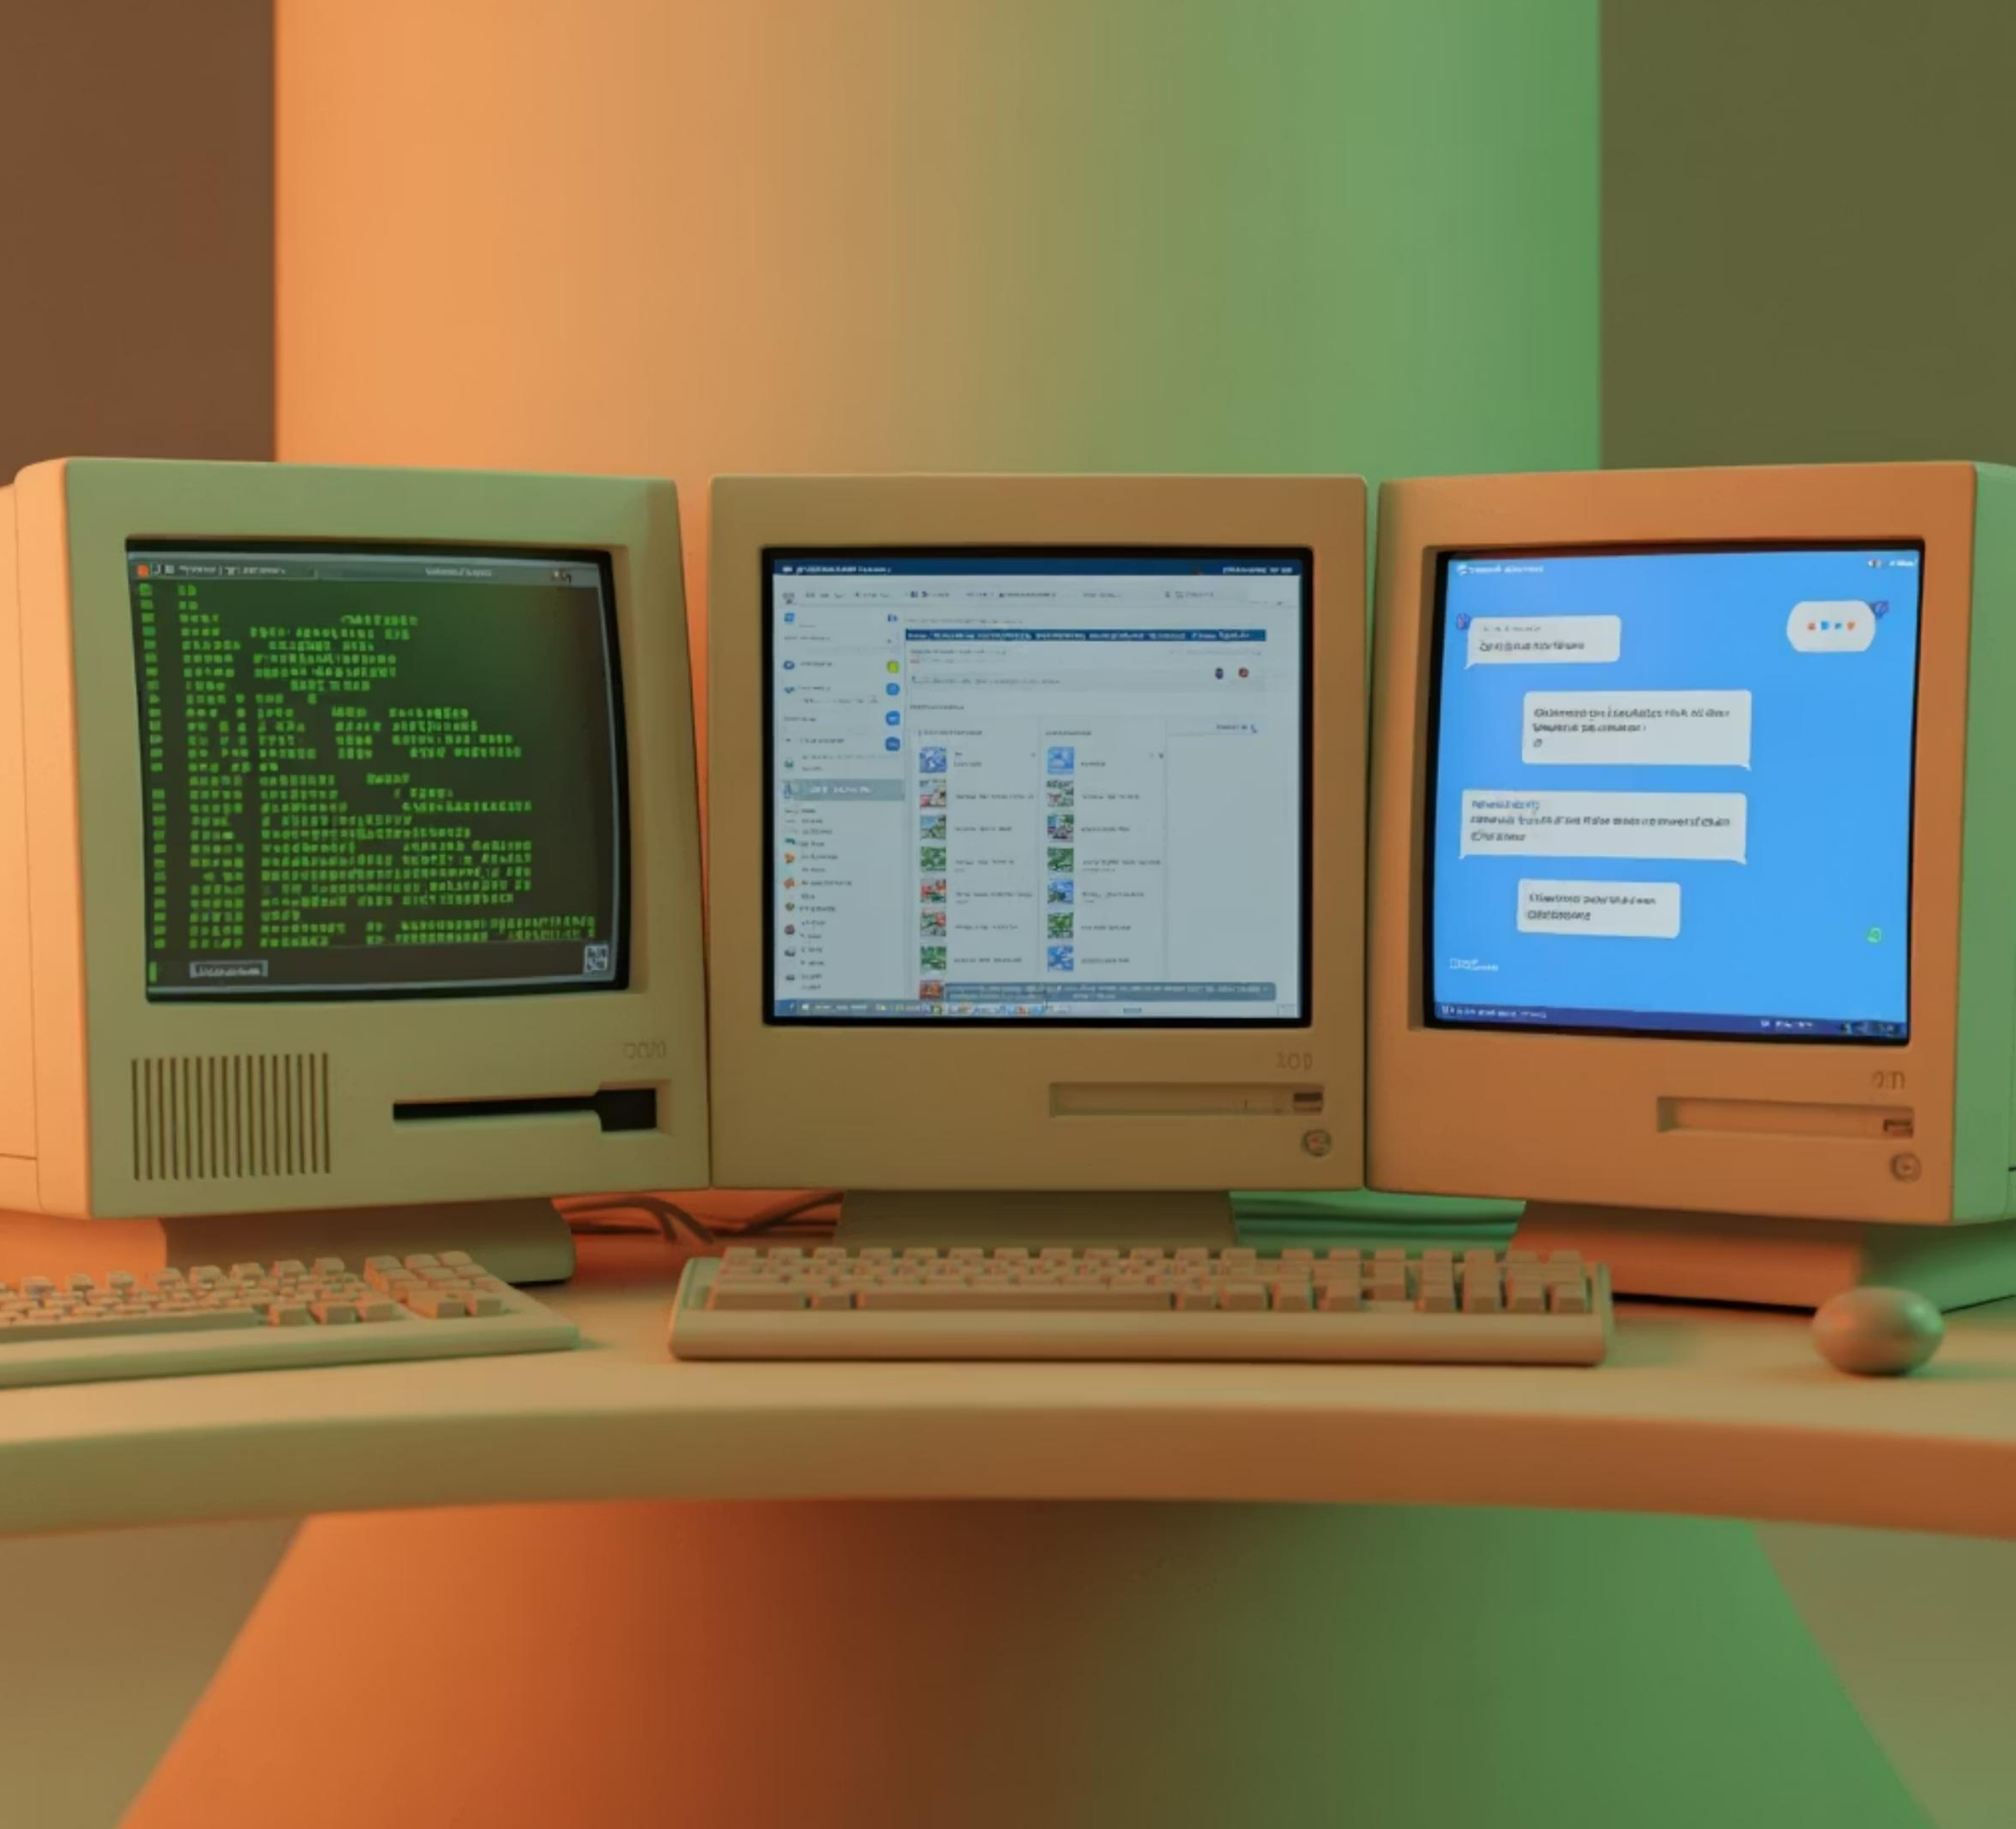
\includegraphics[width=0.85\textwidth]{images/ui-evolution-monitors.png}
\end{center}
\end{frame}

\begin{frame}{Example: Rice Data Portal}
The \href{https://data-portal.rice-business.org}{Rice Data Portal} is an agent.
\vspace{0.3cm}
\begin{itemize}
  \item \textbf{LLM:} ChatGPT --- interprets your natural-language question and writes a SQL query
  \item \textbf{Tool:} A database server in the cloud holding stock-market and financial data
  \item \textbf{Agent:} An app running elsewhere in the cloud that coordinates communication between ChatGPT and the database
\end{itemize}
\vspace{0.3cm}
You type a question (\textit{``Show me AAPL closing prices for 2024''}).  The agent sends it to ChatGPT, which returns a SQL query.  The agent runs the query against the database, sends the results back to ChatGPT for formatting, and displays the answer.  If the query fails, ChatGPT rewrites it and tries again --- multiple rounds, no human intervention.
\end{frame}

\end{document}
